%!TEX root = ../hutbthesis_main.tex

\chapter{着陆控制动力学模型与仿真模型建立}

\section{建模假设与着陆阶段等效模型构建}

为了能够更方便地对固定翼飞行器着陆控制过程展开分析，在不影响主要研究结论的状况下，本文针对实际着陆过程做了适度简化。建模之时主要有以下这些假设：把飞行器当作刚体看待，将机体弹性变形的影响予以忽略，着重分析着陆阶段的纵向运动、侧向运动，把高频小扰动忽略掉，起落架接地之后的缓冲作用通过等效形式来展现，不对内部复杂结构进行细致求解，人机交互强化主要借助状态提示、风险告警、操纵辅助、约束保护来体现，其作用借助控制输入变化反映至飞行状态当中。

鉴于着陆任务所具有的特点，此篇论文把着陆过程划分成了四个阶段，分别是进近段、拉平段、接地区域、滑跑段。在进近段这个阶段，主要达成的任务是下滑轨迹跟踪、速度控制。拉平段这个阶段，主要做的是降低下沉率、调整俯仰姿态。接地区域着重关注的是接地高度、姿态、冲击情况。而滑跑段主要进行的是对接地后的方向保持予以分析。基于这些情况，本文建立了着陆阶段等效模型，把速度、离地高度、下沉率、俯仰角、滚转角、航向角、侧偏量当作主要状态量，将油门、升降舵、副翼、方向舵、襟翼作为主要控制输入量。状态向量可表示为式~\eqref{eq:state-vector}：
\begin{equation}
\boldsymbol{x}=[h_{agl}, V, V_s, \theta, \phi, \psi, e_y]^T
\label{eq:state-vector}
\end{equation}
控制输入向量可表示为式~\eqref{eq:control-vector}：
\begin{equation}
\boldsymbol{u}=[T, \delta_e, \delta_a, \delta_r, \delta_f]^T
\label{eq:control-vector}
\end{equation}

为了展现外部环境对着陆控制所产生的影响，在本论文的模型当中增添了地形因素，把地形划分成诸如平坦地形、起伏地形、山脊地形、谷地地形、阶跃地形等多种类型，以此来对不同地形条件下飞行器着陆过程的响应变化展开分析。齐浩等人指出，飞机起落架落震动力学建模需要全面考量接地瞬态、工况变化，唯有如此，才能确保模型能够比较真实地体现着陆过程中的响应特点。基于此，本论文采用``飞行轨迹模型+地形环境模型+接地边界约束''这种方式来建立着陆阶段等效模型。

\begin{figure}[H]
\centering
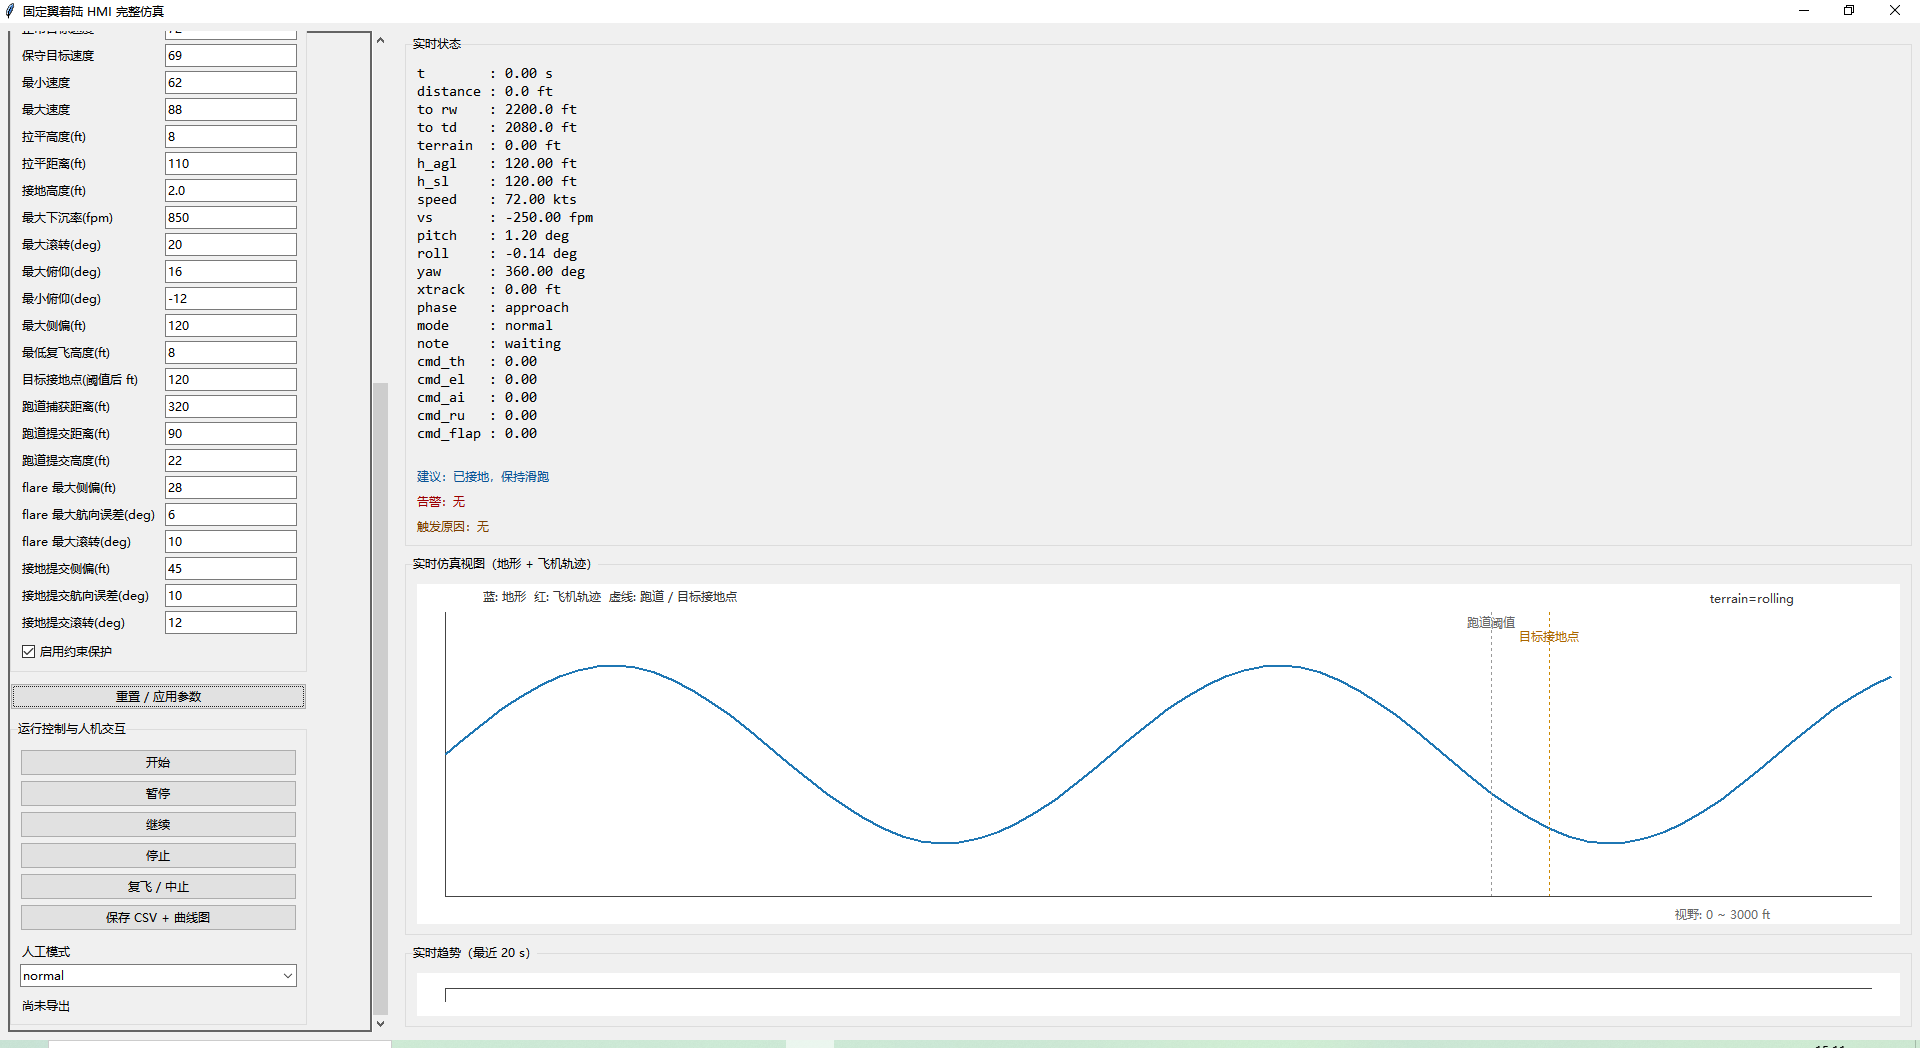
\includegraphics[width=4.19in,height=0.66\textheight,keepaspectratio]{images/image5.png}
\caption{固定翼着陆控制HMI仿真平台界面}
\label{fig:3-1}
\end{figure}

图~\ref{fig:3-1}为本文搭建的固定翼着陆控制仿真平台界面。界面主要包括参数输入区、运行控制区、实时状态显示区以及地形与轨迹显示区，可用于完成参数设置、过程监视和结果分析。

\section{数学模型与输出量定义}

基于上述等效模型，本文建立了纵向运动模型、侧向运动模型。纵向模型着重对飞行器在着陆进程里的速度、高度、下沉率还有俯仰角的变化予以描述，侧向模型主要针对滚转角、航向角、侧偏量的变化展开描述。结合仿真平台的相关参数，本文把下滑角设定为3.0$^\circ$，正常目标速度确定为72
kts，保守目标速度设定成69 kts，最小安全速度规定为62
kts，最大速度设置为88 kts，将拉平高度设定为8 ft，拉平距离定为110
ft，接地高度设为2 ft。这些参数足以满足本文着陆控制仿真分析的需求。

本文针对侧向控制参数设定了边界条件。把最大滚转角定为20$^\circ$，最大俯仰角确定为16$^\circ$，最小俯仰角设定成-12$^\circ$，最大侧偏量设为120
ft。当进入接地区域之后，系统采取更为严格的对准、姿态约束，以此提高着陆的安全性与稳定性。通过这样的做法，模型不但能够反映飞行器进近阶段的纠偏能力，还能够体现近地阶段对平稳接地的要求。

基于论文研究的具体内容，本文把输出量划分成了三类。其一为飞行状态量，其中涵盖了时间、距离、离地的高度、速度、下沉率、俯仰角、滚转角、航向角、侧偏量。其二是控制指令量，具体有油门、升降舵、副翼、方向舵、襟翼指令。其三是交互信息量，包括飞行阶段、提示信息、告警信息、触发原因等。梅荣于无人机起落架着陆缓冲性能优化及试验验证研究里提到，着陆分析需要同时关注飞行状态、接地品质，以此提高仿真结果的完整性。于是，本文在定义输出量的时候兼顾了飞行状态分析与交互提示分析这两方面的内容。

\begingroup\small
\begin{longtable}{@{}
  >{\raggedright\arraybackslash}p{(\columnwidth - 4\tabcolsep) * \real{0.3333}}
  >{\raggedright\arraybackslash}p{(\columnwidth - 4\tabcolsep) * \real{0.3334}}
  >{\raggedright\arraybackslash}p{(\columnwidth - 4\tabcolsep) * \real{0.3334}}@{}}
\caption{仿真平台主要参数设置}\label{tab:3-1}\\
\toprule\noalign{}
\begin{minipage}[b]{\linewidth}\raggedright
参数名称
\end{minipage} & \begin{minipage}[b]{\linewidth}\raggedright
数值
\end{minipage} & \begin{minipage}[b]{\linewidth}\raggedright
单位
\end{minipage} \\
\midrule\noalign{}
\endhead
\bottomrule\noalign{}
\endlastfoot
初始离地高度 & 120 & ft \\
初始速度 & 72 & kts \\
初始下降率 & -250 & fpm \\
下滑角 & 3.0 & $^\circ$ \\
正常目标速度 & 72 & kts \\
保守目标速度 & 69 & kts \\
最小安全速度 & 62 & kts \\
最大允许速度 & 88 & kts \\
拉平高度 & 8 & ft \\
拉平距离 & 110 & ft \\
接地高度 & 2 & ft \\
最大下沉率约束 & 850 & fpm \\
最大滚转角 & 20 & $^\circ$ \\
最大俯仰角 & 16 & $^\circ$ \\
最小俯仰角 & -12 & $^\circ$ \\
最大侧偏量 & 120 & ft \\
\end{longtable}
\endgroup

表~\ref{tab:3-1}为本文仿真平台采用的主要参数设置。这些参数用于统一各工况下的分析条件，为后续工况比较提供基础。

\section{仿真平台实现与参数化设置}

为了验证模型的有效性，本文依据已有的程序搭建了固定翼飞行器着陆控制仿真平台。这个平台拥有参数输入、控制计算、状态刷新、实时显示、数据导出还有结果绘图等功能，可以满足着陆控制系统仿真分析的需求。平台整体是由参数设置模块、控制器模块、环境与地形模块、状态显示模块、结果输出模块构成的，其中参数设置模块用来输入飞行初始条件和控制边界，控制器模块负责实时生成控制指令，环境模块承担建立不同地形条件的任务，结果输出模块用于保存CSV数据和仿真曲线图。

通过结合上传的仿真结果能够发现，不同地形条件下飞行器的着陆过程有着显著不同。在平坦地形时，AGL曲线整体下降比较平稳，速度、姿态的变化同样比较平顺，处于起伏地形和山脊地形时，离地高度变化更快，姿态修正更为频繁，谷地和阶跃地形会对近地区域的高度判断、拉平时机造成影响。这显示出复杂地形会加大着陆控制的难度，也进一步表明在人机交互强化条件下展开仿真分析是很有必要的。

\begin{figure}[H]
\centering
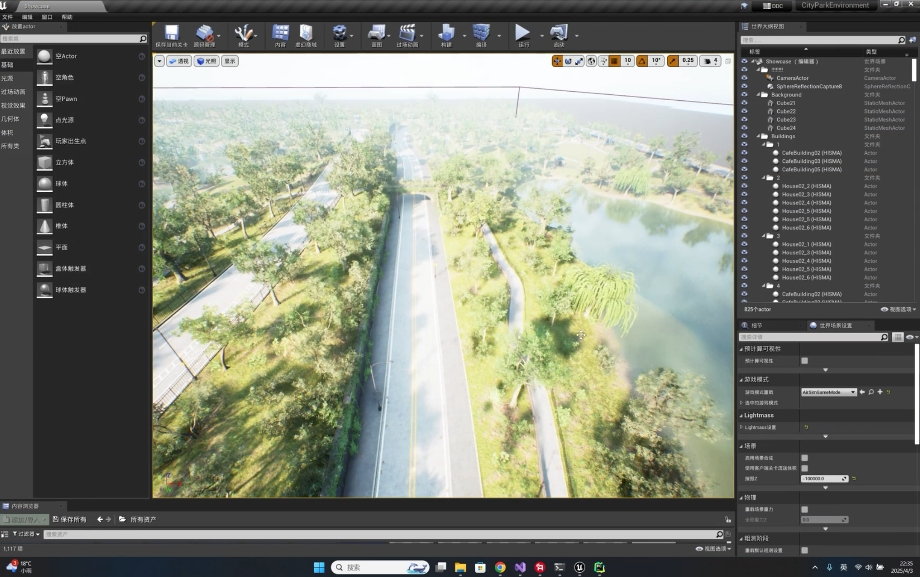
\includegraphics[width=0.92\linewidth,height=0.66\textheight,keepaspectratio]{images/image6.jpg}
\caption{仿真平台搭建}
\label{fig:3-2}
\end{figure}

\begin{figure}[H]
\centering
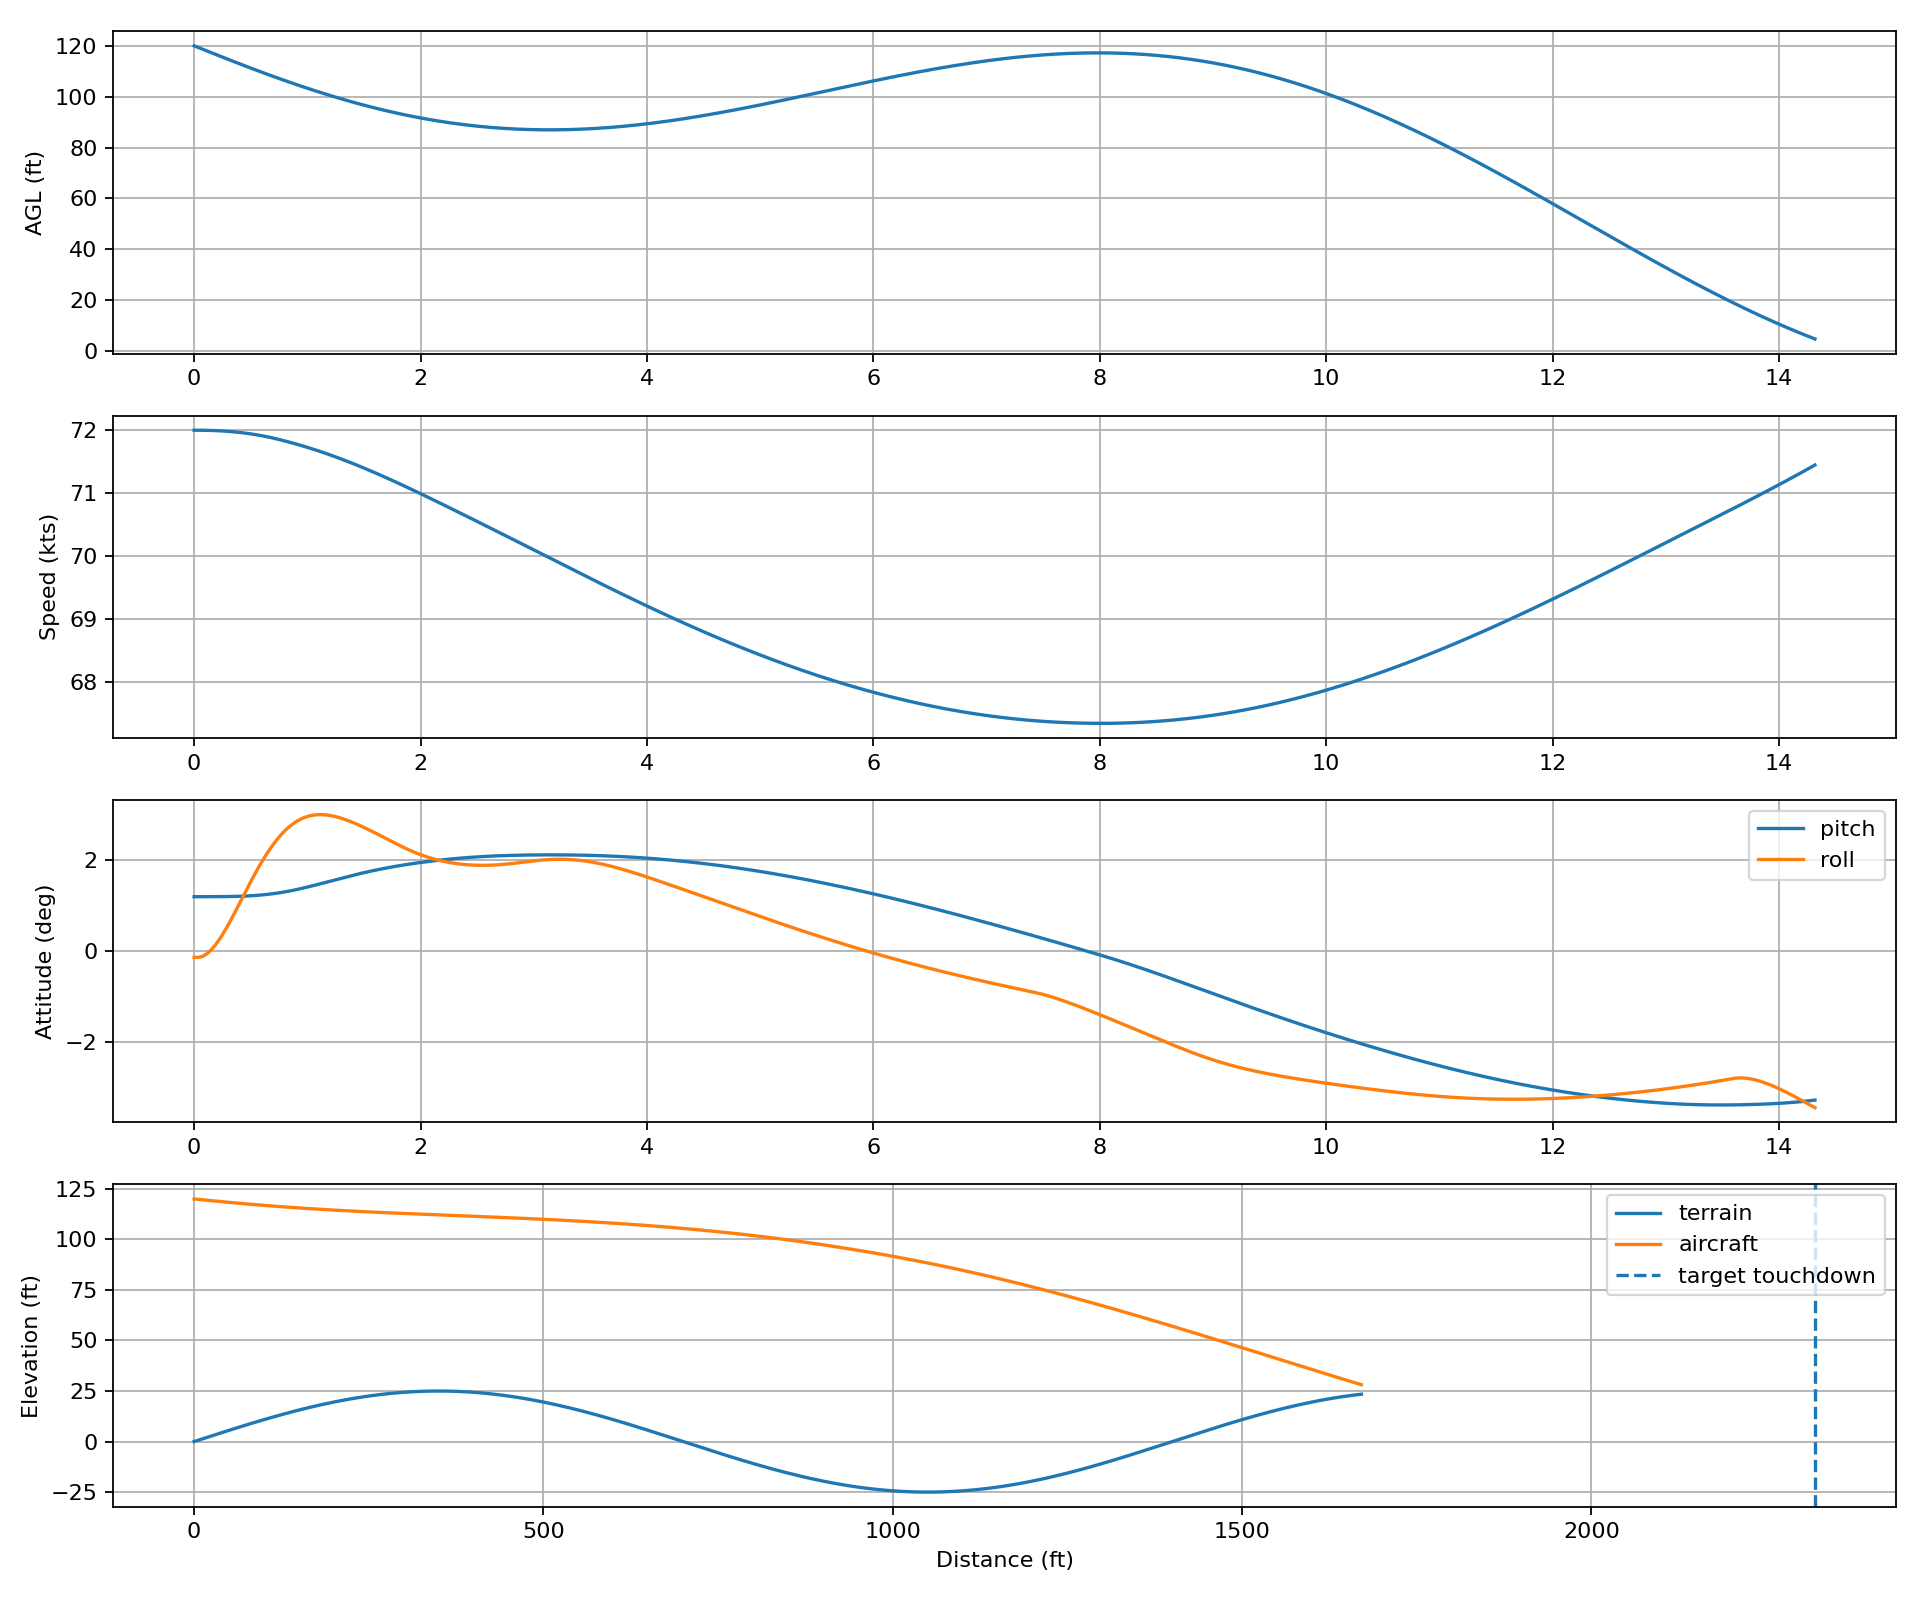
\includegraphics[width=4.00in,height=0.66\textheight,keepaspectratio]{images/image7.png}
\caption{平坦地形基准工况仿真结果}
\label{fig:3-3}
\end{figure}

图~\ref{fig:3-3}表明，在平坦地形工况下，飞行器着陆过程整体较为平稳，适合作为后续工况对比分析的基准工况。

\begin{figure}[H]
\centering
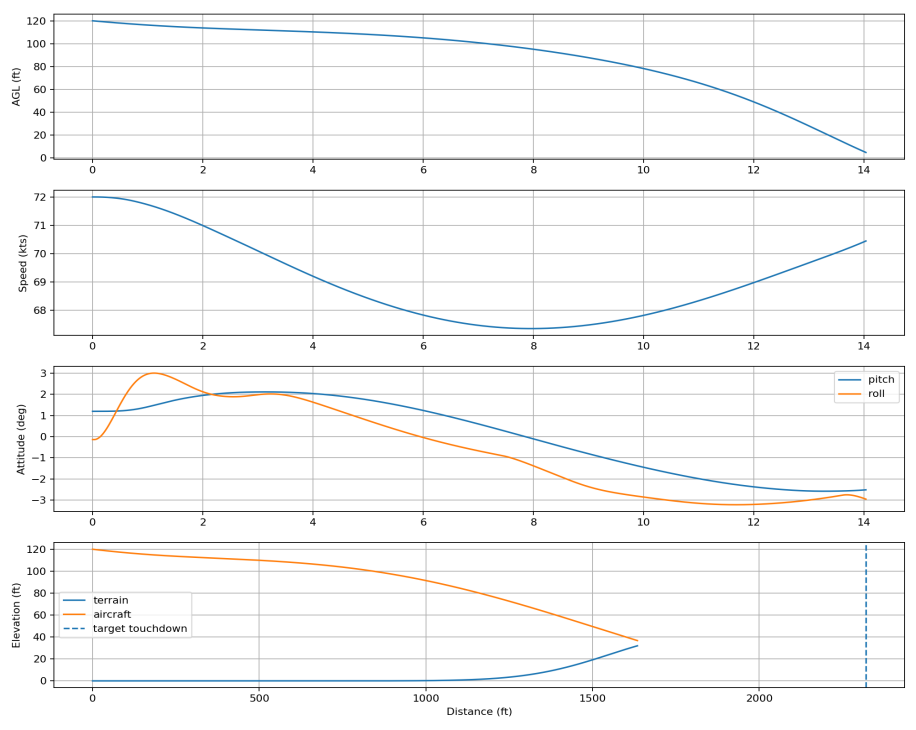
\includegraphics[width=4.16in,height=0.66\textheight,keepaspectratio]{images/image8.png}
\caption{起伏地形工况仿真结果}
\label{fig:3-4}
\end{figure}

图~\ref{fig:3-4}显示，起伏地形会使飞行器相对离地高度变化更加明显，从而增加着陆后段的控制难度。

\begin{figure}[H]
\centering
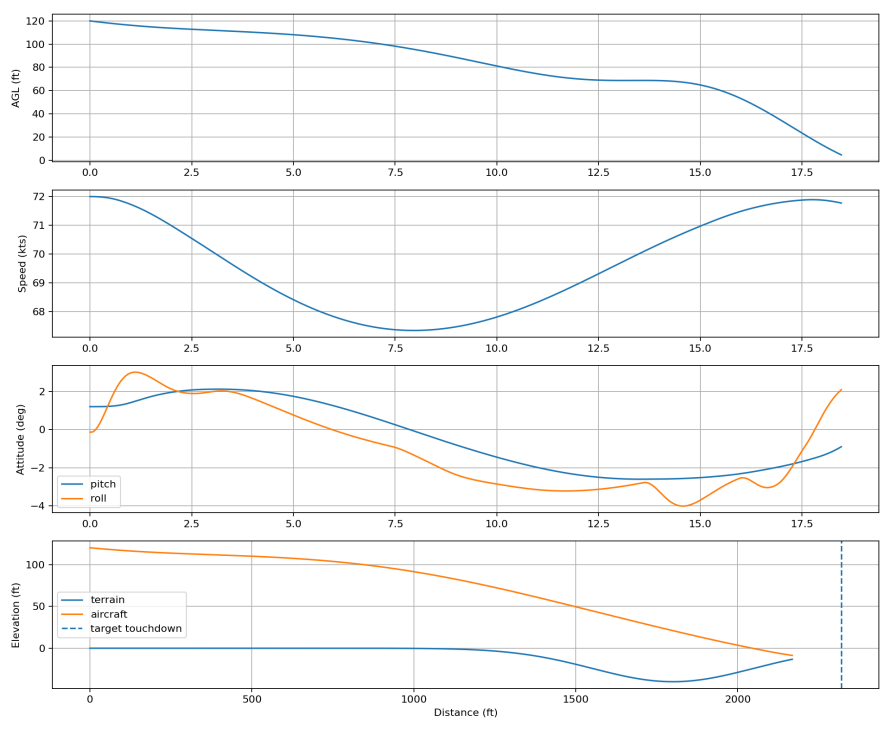
\includegraphics[width=4.05in,height=0.66\textheight,keepaspectratio]{images/image9.png}
\caption{山脊地形工况仿真结果}
\label{fig:3-5}
\end{figure}

图~\ref{fig:3-5}说明，山脊地形会使飞行器在接近着陆区域时面临地形快速抬升，对轨迹保持和姿态修正提出更高要求。

\begin{figure}[H]
\centering
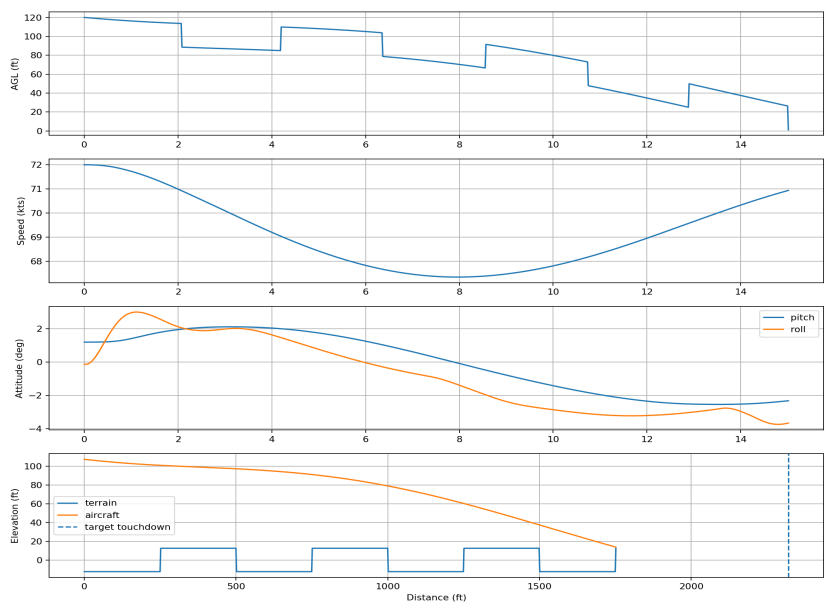
\includegraphics[width=3.79in,height=0.66\textheight,keepaspectratio]{images/image10.png}
\caption{谷地地形工况仿真结果}
\label{fig:3-6}
\end{figure}

图~\ref{fig:3-6}表明，谷地地形会改变飞行器末段离地高度变化规律，使操纵者对拉平时机的判断更加复杂。

\begin{figure}[H]
\centering
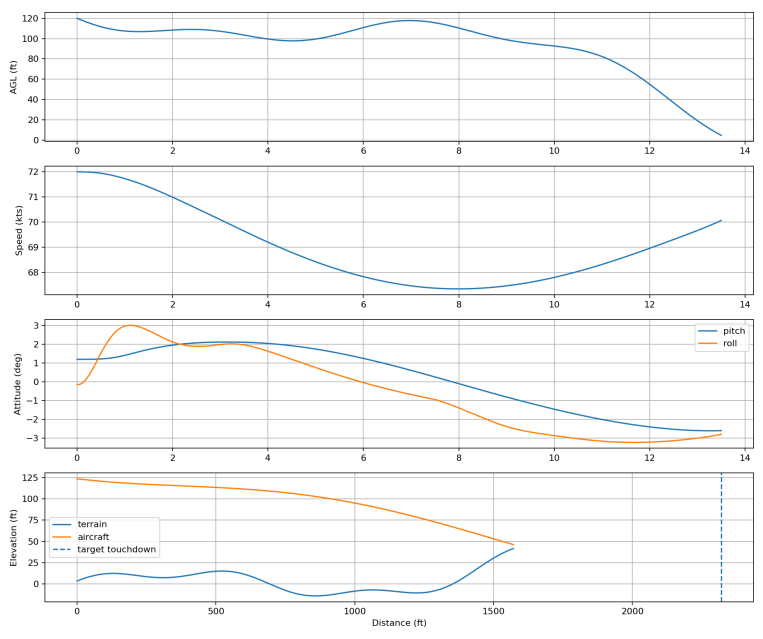
\includegraphics[width=3.47in,height=0.66\textheight,keepaspectratio]{images/image11.png}
\caption{阶跃地形工况仿真结果}
\label{fig:3-7}
\end{figure}

图~\ref{fig:3-7}显示，阶跃地形会使飞行器相对离地高度出现突变特征，从而对着陆阶段的稳定控制产生影响。

为了便于比较不同地形工况下的仿真结果，本文对关键指标进行了整理，如表~\ref{tab:3-2}所示。

\begingroup\small
\begin{longtable}{@{}
  >{\raggedright\arraybackslash}p{(\columnwidth - 10\tabcolsep) * \real{0.1666}}
  >{\raggedright\arraybackslash}p{(\columnwidth - 10\tabcolsep) * \real{0.1666}}
  >{\raggedright\arraybackslash}p{(\columnwidth - 10\tabcolsep) * \real{0.1666}}
  >{\raggedright\arraybackslash}p{(\columnwidth - 10\tabcolsep) * \real{0.1666}}
  >{\raggedright\arraybackslash}p{(\columnwidth - 10\tabcolsep) * \real{0.1667}}
  >{\raggedright\arraybackslash}p{(\columnwidth - 10\tabcolsep) * \real{0.1667}}@{}}
\caption{不同地形工况关键仿真结果对比}\label{tab:3-2}\\
\toprule\noalign{}
\begin{minipage}[b]{\linewidth}\raggedright
工况类型
\end{minipage} & \begin{minipage}[b]{\linewidth}\raggedright
仿真时长/s
\end{minipage} & \begin{minipage}[b]{\linewidth}\raggedright
最终AGL/ft
\end{minipage} & \begin{minipage}[b]{\linewidth}\raggedright
末段速度/kts
\end{minipage} & \begin{minipage}[b]{\linewidth}\raggedright
末段俯仰角/($^\circ$)
\end{minipage} & \begin{minipage}[b]{\linewidth}\raggedright
末段滚转角/($^\circ$)
\end{minipage} \\
\midrule\noalign{}
\endhead
\bottomrule\noalign{}
\endlastfoot
平坦地形 & 17.15 & 4.60 & 71.80 & -1.28 & -2.28 \\
起伏地形 & 14.32 & 4.70 & 71.45 & -3.29 & -3.45 \\
山脊地形 & 14.03 & 4.74 & 70.44 & -2.52 & -2.96 \\
谷地地形 & 18.47 & 4.60 & 71.78 & -0.90 & 2.09 \\
阶跃地形 & 15.02 & 1.20 & 70.94 & -2.33 & -3.67 \\
\end{longtable}
\endgroup

由表~\ref{tab:3-2}可以看出，不同地形条件下系统输出结果存在明显差异。起伏地形工况的最大下沉率绝对值最大，说明其对着陆纵向控制影响更突出；谷地地形工况的最大滚转角最大，说明其对姿态控制和横向稳定性影响更明显；阶跃地形工况最终AGL最低，反映出地形突变对末段离地高度判断的干扰最强。因此，在后续工况设计与评价分析中，有必要把复杂地形作为重点考察对象，并结合人机交互强化策略进一步分析其对着陆品质改善的作用。

本文仿真平台在参数配置、控制逻辑方面保留了工程可扩展性。比如说能够进一步借助调整缓冲边界参数、接地阈值、风险触发条件，去模拟不同起落架构型、不同着陆策略之下的响应差异。赵知辛等人在仿竹设计无人机起落架结构中的应用研究显示，起落架系统设计不但关乎结构轻量化，而且对接地吸能、冲击适应能力也有影响。受此启发，本文虽说重点研究的是着陆控制系统与人机交互强化，不过在仿真平台设置里依旧保留了对接地边界、缓冲安全性、复杂地形适应性的关注，进而为后续系统优化分析提供更为完整的基础。
